% Options for packages loaded elsewhere
\PassOptionsToPackage{unicode}{hyperref}
\PassOptionsToPackage{hyphens}{url}
\PassOptionsToPackage{dvipsnames,svgnames,x11names}{xcolor}
%
\documentclass[
  letterpaper,
  DIV=11,
  numbers=noendperiod,
  oneside]{scrartcl}

\usepackage{amsmath,amssymb}
\usepackage{iftex}
\ifPDFTeX
  \usepackage[T1]{fontenc}
  \usepackage[utf8]{inputenc}
  \usepackage{textcomp} % provide euro and other symbols
\else % if luatex or xetex
  \usepackage{unicode-math}
  \defaultfontfeatures{Scale=MatchLowercase}
  \defaultfontfeatures[\rmfamily]{Ligatures=TeX,Scale=1}
\fi
\usepackage{lmodern}
\ifPDFTeX\else  
    % xetex/luatex font selection
\fi
% Use upquote if available, for straight quotes in verbatim environments
\IfFileExists{upquote.sty}{\usepackage{upquote}}{}
\IfFileExists{microtype.sty}{% use microtype if available
  \usepackage[]{microtype}
  \UseMicrotypeSet[protrusion]{basicmath} % disable protrusion for tt fonts
}{}
\makeatletter
\@ifundefined{KOMAClassName}{% if non-KOMA class
  \IfFileExists{parskip.sty}{%
    \usepackage{parskip}
  }{% else
    \setlength{\parindent}{0pt}
    \setlength{\parskip}{6pt plus 2pt minus 1pt}}
}{% if KOMA class
  \KOMAoptions{parskip=half}}
\makeatother
\usepackage{xcolor}
\usepackage[left=1in,marginparwidth=2.0666666666667in,textwidth=4.1333333333333in,marginparsep=0.3in]{geometry}
\setlength{\emergencystretch}{3em} % prevent overfull lines
\setcounter{secnumdepth}{-\maxdimen} % remove section numbering
% Make \paragraph and \subparagraph free-standing
\makeatletter
\ifx\paragraph\undefined\else
  \let\oldparagraph\paragraph
  \renewcommand{\paragraph}{
    \@ifstar
      \xxxParagraphStar
      \xxxParagraphNoStar
  }
  \newcommand{\xxxParagraphStar}[1]{\oldparagraph*{#1}\mbox{}}
  \newcommand{\xxxParagraphNoStar}[1]{\oldparagraph{#1}\mbox{}}
\fi
\ifx\subparagraph\undefined\else
  \let\oldsubparagraph\subparagraph
  \renewcommand{\subparagraph}{
    \@ifstar
      \xxxSubParagraphStar
      \xxxSubParagraphNoStar
  }
  \newcommand{\xxxSubParagraphStar}[1]{\oldsubparagraph*{#1}\mbox{}}
  \newcommand{\xxxSubParagraphNoStar}[1]{\oldsubparagraph{#1}\mbox{}}
\fi
\makeatother


\providecommand{\tightlist}{%
  \setlength{\itemsep}{0pt}\setlength{\parskip}{0pt}}\usepackage{longtable,booktabs,array}
\usepackage{calc} % for calculating minipage widths
% Correct order of tables after \paragraph or \subparagraph
\usepackage{etoolbox}
\makeatletter
\patchcmd\longtable{\par}{\if@noskipsec\mbox{}\fi\par}{}{}
\makeatother
% Allow footnotes in longtable head/foot
\IfFileExists{footnotehyper.sty}{\usepackage{footnotehyper}}{\usepackage{footnote}}
\makesavenoteenv{longtable}
\usepackage{graphicx}
\makeatletter
\def\maxwidth{\ifdim\Gin@nat@width>\linewidth\linewidth\else\Gin@nat@width\fi}
\def\maxheight{\ifdim\Gin@nat@height>\textheight\textheight\else\Gin@nat@height\fi}
\makeatother
% Scale images if necessary, so that they will not overflow the page
% margins by default, and it is still possible to overwrite the defaults
% using explicit options in \includegraphics[width, height, ...]{}
\setkeys{Gin}{width=\maxwidth,height=\maxheight,keepaspectratio}
% Set default figure placement to htbp
\makeatletter
\def\fps@figure{htbp}
\makeatother

<style>
 .title {
  font-size: 2.0em;
}
</style>
<style>
.center-xy {
  margin: 0;
  position: absolute;
  top: 50%;
  left: 20%;
  -ms-transform: translateY(-50%), translateX(-50%);
  transform: translateY(-50%), translateX(-50%);
}
</style>
\KOMAoption{captions}{tableheading}
\makeatletter
\@ifpackageloaded{tcolorbox}{}{\usepackage[skins,breakable]{tcolorbox}}
\@ifpackageloaded{fontawesome5}{}{\usepackage{fontawesome5}}
\definecolor{quarto-callout-color}{HTML}{909090}
\definecolor{quarto-callout-note-color}{HTML}{0758E5}
\definecolor{quarto-callout-important-color}{HTML}{CC1914}
\definecolor{quarto-callout-warning-color}{HTML}{EB9113}
\definecolor{quarto-callout-tip-color}{HTML}{00A047}
\definecolor{quarto-callout-caution-color}{HTML}{FC5300}
\definecolor{quarto-callout-color-frame}{HTML}{acacac}
\definecolor{quarto-callout-note-color-frame}{HTML}{4582ec}
\definecolor{quarto-callout-important-color-frame}{HTML}{d9534f}
\definecolor{quarto-callout-warning-color-frame}{HTML}{f0ad4e}
\definecolor{quarto-callout-tip-color-frame}{HTML}{02b875}
\definecolor{quarto-callout-caution-color-frame}{HTML}{fd7e14}
\makeatother
\makeatletter
\@ifpackageloaded{caption}{}{\usepackage{caption}}
\AtBeginDocument{%
\ifdefined\contentsname
  \renewcommand*\contentsname{Table of contents}
\else
  \newcommand\contentsname{Table of contents}
\fi
\ifdefined\listfigurename
  \renewcommand*\listfigurename{List of Figures}
\else
  \newcommand\listfigurename{List of Figures}
\fi
\ifdefined\listtablename
  \renewcommand*\listtablename{List of Tables}
\else
  \newcommand\listtablename{List of Tables}
\fi
\ifdefined\figurename
  \renewcommand*\figurename{Figure}
\else
  \newcommand\figurename{Figure}
\fi
\ifdefined\tablename
  \renewcommand*\tablename{Table}
\else
  \newcommand\tablename{Table}
\fi
}
\@ifpackageloaded{float}{}{\usepackage{float}}
\floatstyle{ruled}
\@ifundefined{c@chapter}{\newfloat{codelisting}{h}{lop}}{\newfloat{codelisting}{h}{lop}[chapter]}
\floatname{codelisting}{Listing}
\newcommand*\listoflistings{\listof{codelisting}{List of Listings}}
\makeatother
\makeatletter
\makeatother
\makeatletter
\@ifpackageloaded{caption}{}{\usepackage{caption}}
\@ifpackageloaded{subcaption}{}{\usepackage{subcaption}}
\makeatother
\makeatletter
\@ifpackageloaded{sidenotes}{}{\usepackage{sidenotes}}
\@ifpackageloaded{marginnote}{}{\usepackage{marginnote}}
\makeatother

\ifLuaTeX
  \usepackage{selnolig}  % disable illegal ligatures
\fi
\usepackage{bookmark}

\IfFileExists{xurl.sty}{\usepackage{xurl}}{} % add URL line breaks if available
\urlstyle{same} % disable monospaced font for URLs
\hypersetup{
  pdftitle={開発経済論中間試験},
  colorlinks=true,
  linkcolor={blue},
  filecolor={Maroon},
  citecolor={Blue},
  urlcolor={Blue},
  pdfcreator={LaTeX via pandoc}}


\title{開発経済論中間試験}
\usepackage{etoolbox}
\makeatletter
\providecommand{\subtitle}[1]{% add subtitle to \maketitle
  \apptocmd{\@title}{\par {\large #1 \par}}{}{}
}
\makeatother
\subtitle{聖心女子大学国際交流学科\\
2024年秋学期}
\author{}
\date{}

\begin{document}
\maketitle

<script type="text/x-mathjax-config">
MathJax.Hub.Config({
  TeX: {
    Macros: {
      E: "{\\Large\\varepsilon}",
      NU: "{\\Large\\nu}",
      SIM: "{\\large\\stackrel{\\small +}{\\sim}}",
      SIMpos: "{\\large\\stackrel{\\small +}{\\sim}}",
      SIMneg: "{\\large\\stackrel{\\small -}{\\sim}}",
      bfv: "{\\mathbf{v}}",
      bfV: "{\\mathbf{V}}",
      bfw: "{\\mathbf{w}}",
      bfW: "{\\mathbf{W}}",
      bfx: "{\\mathbf{x}}",
      bfX: "{\\mathbf{X}}",
      bfalpha: "{\\boldsymbol{\\alpha}}",
      bfbeta: "{\\boldsymbol{\\beta}}",
      bfgamma: "{\\boldsymbol{\\gamma}}",
      cov: "{\\mbox{cov}}",
      corr: "{\\mathrm{corr}}",
      st: "{\\mbox{s.t.}}"
    }
  }
});
</script>


\subsection{ジェンダー教育実験}\label{ux30b8ux30a7ux30f3ux30c0ux30fcux6559ux80b2ux5b9fux9a13}

世界銀行では、イスラム教信者の多い国でジェンダー教育を進めました。イスラム教徒が大半を占める国では、女性と男性の権利が著しく不平等だからです。とあるプログラムでは、高位のイマム(聖職者)が各モスクに所属している信者向けに「ジェンダー教育に参加するように」というテキスト・メッセージを(ショート・メッセージ・サービスSMSで)送りました。

\begin{enumerate}
\def\labelenumi{\arabic{enumi}.}
\tightlist
\item
  イマムがテキスト・メッセージを送ることの効果を計測するには、どのような実験が必要でしょうか。
\item
  女性の権利擁護のプログラムやイベントは、以下のa.とb.では効果が違うかもしれません。a.とb.の効果の違いを計測するには、どのような実験デザインにすべきでしょうか。

  \begin{enumerate}
  \def\labelenumii{\alph{enumii}.}
  \tightlist
  \item
    女性だけを対象にして実施するとき
  \item
    男女を対象にするとき
  \end{enumerate}
\end{enumerate}

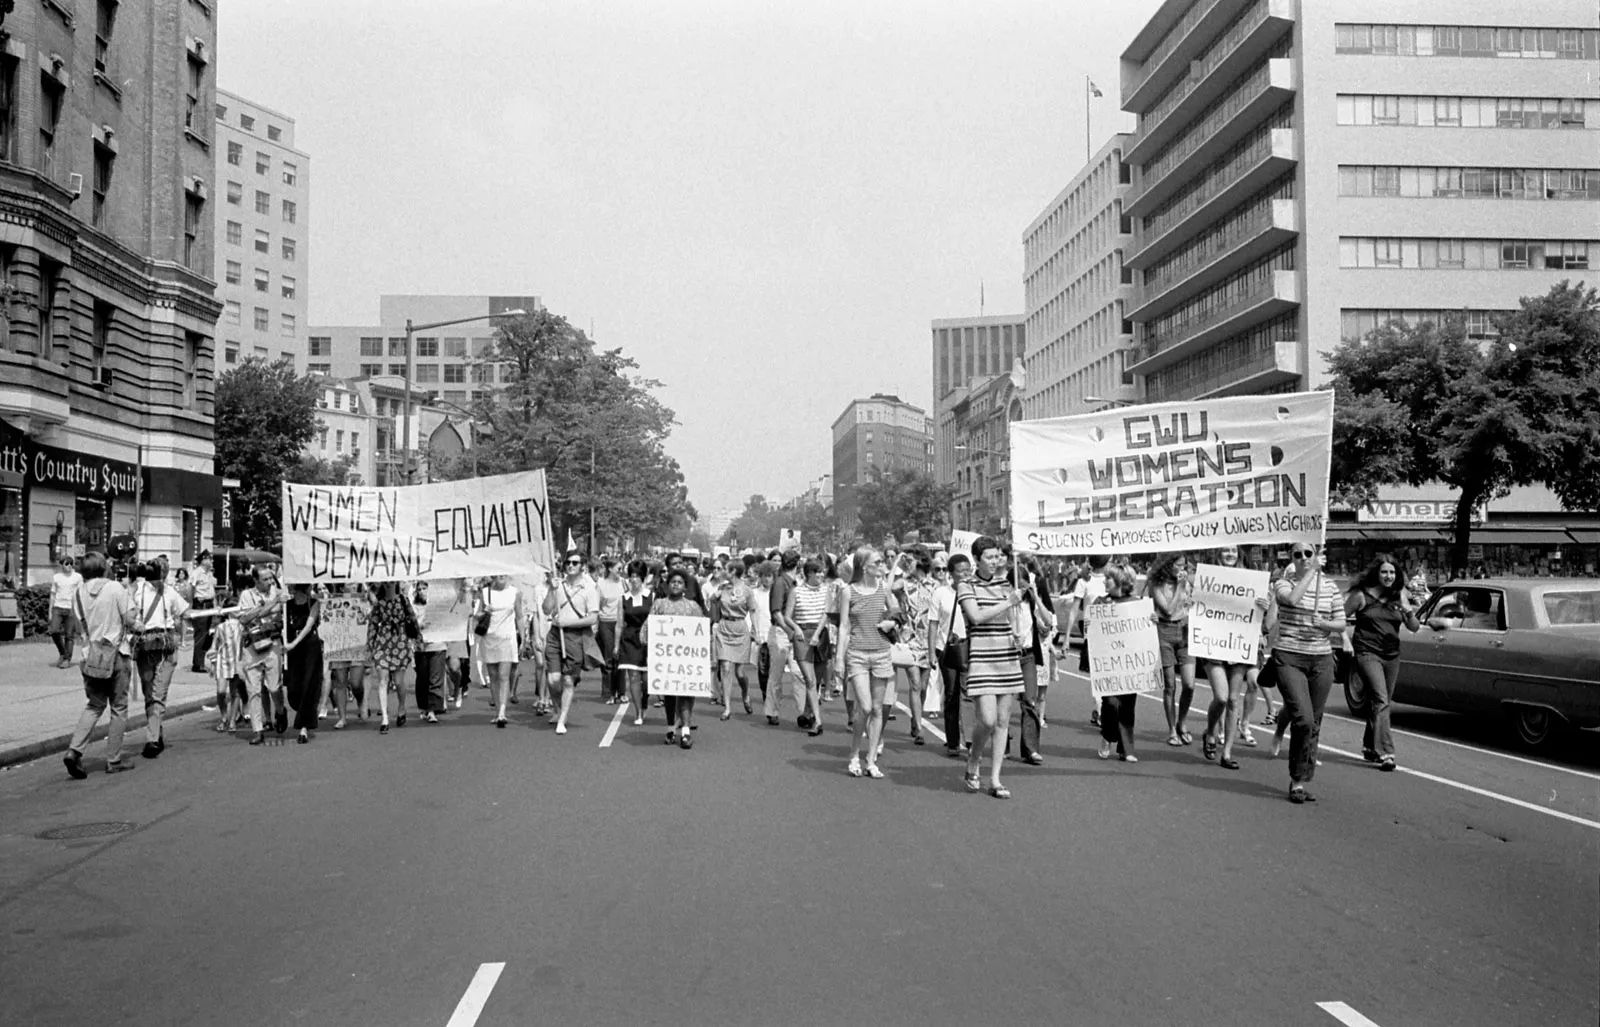
\includegraphics{DC1970.jpg}\{width = ``50\%''\}

U.S. News \& World Report Magazine/Library of Congress, Washington, D.C.
(digital. id. ppmsca 03425)

\subsection{09回講義へのRP}\label{ux56deux8b1bux7fa9ux3078ux306erp}

\begin{tcolorbox}[enhanced jigsaw, bottomrule=.15mm, leftrule=.75mm, arc=.35mm, toprule=.15mm, colback=white, rightrule=.15mm, breakable, left=2mm, opacityback=0, colframe=quarto-callout-note-color-frame]

最近のニュースだと「ワールドツアーを行うテイラースウィフトによる経済効果」がニュースとなっていた。米旅行協会によると、ツアーに伴う支出を含み、テイラーは米国内での公演5ヶ月で100億ドル以上の経済効果をもたらしたとされている。実際に日本公演でも、経済効果として341億円を記録したと毎日新聞が報道していた。テロとは異なる観点だが、こうした世界的アーティストによる経済効果、経済成長への影響についてもっと調べてみたいと感じた。

\end{tcolorbox}

テイラー・スウィフトの日本ツアー経済効果はどのようにして計測できるでしょうか。以下の問いに答えながら、最後の問いでどのように計測するか答えてください。

\begin{enumerate}
\def\labelenumi{\arabic{enumi}.}
\tightlist
\item
  通常は(ツアーによる)支出拡大を経済効果といいます。つまり、ツアーありのときの支出-ツアー無しのときの支出、が経済効果です。どのようなデータ(支出項目)を使うべきでしょうか。どのようなデータがどのくらいの頻度で公開されているのか調べて支出項目を挙げてください。
\item
  東京都市大学の江頭氏の推計は、Bloombergによると
\end{enumerate}

\begin{quote}
チケット、グッズ、観光消費、事業費などを含めて算出した
\end{quote}

そうです。詳細は不明ですが、CF=ゼロ円、と想定している可能性が高いです。このCFの現実妥当性を述べてください。

\begin{enumerate}
\def\labelenumi{\arabic{enumi}.}
\setcounter{enumi}{2}
\tightlist
\item
  あなたならば、どのような方法で経済効果を推計しますか。どのようにしてCFを得るのか明示して答えてください。
\end{enumerate}




\end{document}
